\section{Dit comme ça...}

\subsection{Phénomènes d'induction}
\subsubsection{Loi de Lentz}
    La \textbf{Nature aime la stabilité}. La représentation faite par la Physique d’un
    système tend toujours à assurer la stabilité en passant d’un état d’équilibre
    à un autre. Comme par exemple le fait de tordre un bout de métal. On peut
    croire que rien ne s’est passé mais que nenni ! Il y eu un transfert de chaleur
    comme \textbf{réaction pour restaurer la stabilité}. \\
    On comprend plus aisément ce qui va suivre. Quand un courant variable parcourt un circuit , il y a apparition d’un champ qui s’oppose aux variations de
    courant pour restaurer la stabilité (d’où opposition de phase visible sur oscilloscope) .

    \begin{theo}[Loi de Lentz]{thm:lentz}
        La circulation sur un contour fermé du champ électrique agit comme l'opposé de la variation du flux par rapport au temps.
        \[
        \oint_C \overrightarrow{E}.\overrightarrow{dl} = e = - \ddt{\Phi}
        \]
    \end{theo}

\subsubsection{Théorème de Gauss}
    \begin{theo}[Forme globale]{thm:gaussG}
        Le flux du champ électrique à travers une surface fermée quelconque (que l’on
    appelle surface de Gauss) est le produit de l’inverse de la perméabilité du vide par
    la charge algébrique totale.
        \[
        \Phi_E = \frac{1}{\epsilon_0} \iiint_V \rho \,d\tau = \frac{Q_{int}}{\epsilon_0}
        \]
        \begin{center}
            Forme globale (intégrale) \textbf{macroscopique}
        \end{center}
    Avec $\rho = \pp{Q}{\tau}$, la densité volumique de charge.
    \end{theo}

\subsection{Vous avez dit potentiel ?}
Le potentiel est une grandeur physique qui favorise la naissance d’une force
(différence potentiel $\Rightarrow$ force). On peut comprendre ce concept par la gravitation :
Placez un ballon sur un endroit haut d’une pente, une force naîtra et tendra à
amener ce ballon vers le bas de la pente. Cette force est née de par la différence
de hauteur qui existait. Ici, le potentiel est l’altitude. Et physiquement, on mesure
cette différence d’altitude ! (Il va donc de même pour l’électrostatique)

\subsection{Des bras et des kets}
$\braket{\varphi|\psi}$, $\bra{\varphi}$ , $\ket{\psi}$ , $\ket{\varphi}\bra{\psi}$

Le produit tensoriel de deux qbits donne:
\begin{equation}
    \ket{0}\otimes\ket{1}=
    \begin{pmatrix}
        1\\
        0
    \end{pmatrix}
    \otimes
    \begin{pmatrix}
        0\\
        1
    \end{pmatrix}
    =
    \begin{pmatrix}
        1 \begin{pmatrix}
            0\\
            1
        \end{pmatrix}
        \\ \\
        0 \begin{pmatrix}
            0\\
            1
        \end{pmatrix}
    \end{pmatrix}
    =
    \begin{pmatrix}
        0\\
        1\\
        0\\
        0
    \end{pmatrix}
    =\ket{01}
\end{equation}

\subsection{Une matrice}
\[
  N\textrm{ lignes}
  \stackrel{\mbox{$M$ colonnes}}{%
    \begin{bmatrix}
    a_{11} & a_{12} & \cdots & a_{1M} \\
    a_{21} & a_{22} & \cdots & a_{2M} \\
    \vdots & \vdots & \ddots & \vdots \\
    a_{N1} & a_{N2} & \cdots & a_{NM}
    \end{bmatrix}%
  }\ \quad
  \stackrel{\stackrel{\mbox{tout plein de}}{\mbox{bisous}}}{%
    \begin{bmatrix}
    bisou_1 \\
    bisou_2 \\
    \vdots \\
    bisou_N
    \end{bmatrix}%
   }
\]

\subsection{Une autre sous-section}
Il est aussi intéréssant de bien référencer nos dires.  Je veux bien croire que vous êtes très
intelligent mais on puise forcément l'eau d'une source. Avec \texttt{biblatex}, on peut afficher une
bibliographie propre divisée en sections, en fonction du style de la citation !

Un article sur la formation du citoyen soldat sous la République
jacobine\footnote{\cite{guiragossian:hal-02115427}}. Puis on a de très bons liens Wikipédia tel que
le portail de Cryptologie\footnote{\cite{crypto}}. Ainsi qu'un livre à absolument lire pour
comprendre les couches réseaux et les protocoles associées\footnote{\cite{topdown}}.

Ci-contre la méthode pour utiliser une note de bas de page au sein même d'une caption de figure :

\begin{figure}[H]
    \centering
    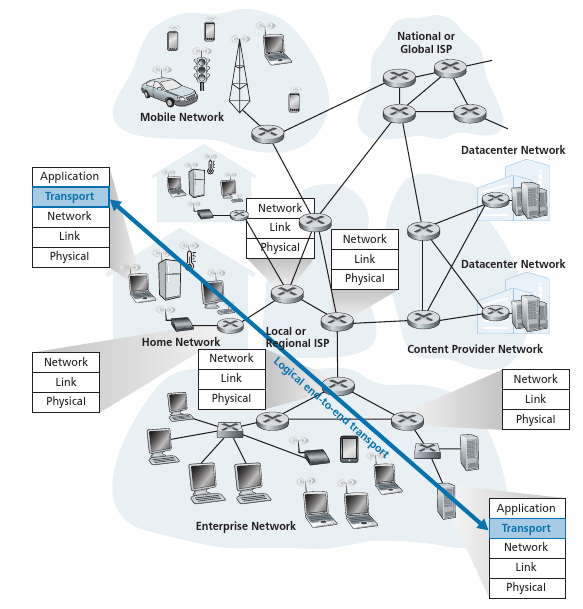
\includegraphics[width=\textwidth]{logicaltcp.png}
    \caption[Communication logique via la couche Transport]{Communication logique via la couche Transport\protect\footnotemark}
    \label{logicalT}
\end{figure}

\footnotetext{\cite{topdown}}